\documentclass[a4paper,10pt]{article}

\usepackage[utf8]{inputenx}
\usepackage[style=apa,backend=biber,alldates=iso8601,doi=false]{biblatex}
\usepackage[nottoc,notlot,notlof]{tocbibind}
\usepackage[font=small, labelfont=bf]{caption}
\usepackage[toc, page]{appendix}
\usepackage{hyperref}
\usepackage[braket, qm]{qcircuit}
\usepackage{a4wide}
\usepackage{enumitem}
\usepackage{fancyhdr}
\usepackage{blochsphere}
\usepackage{xcolor}
\usepackage{amssymb}
\usepackage{amsmath}
\usepackage{multirow}
\usepackage{subcaption}
\usepackage{multicol}
\usepackage{dirtytalk}
\usepackage{tikz-3dplot}
\usepackage[outline]{contour}
\usepackage{cprotect}
\usetikzlibrary{3d}

\hypersetup{
	colorlinks,
	linkcolor={red!90!black},
	citecolor={green!90!black},
	urlcolor={magenta!90!black}
}

\newbibmacro{string+doi}[1]{%
	\iffieldundef{doi}{#1}{\href{http://dx.doi.org/\thefield{doi}}{#1}}}
\DeclareFieldFormat{title}{\usebibmacro{string+doi}{\mkbibemph{#1}}}
\DeclareFieldFormat[article]{title}{\usebibmacro{string+doi}{\mkbibquote{#1}}}

\DeclareLanguageMapping{english}{english-apa}
%\DeclareFieldFormat[article,unpublished,misc,online]{title}{\textit{#1}}

\renewcommand{\abstractname}{Summary}
\renewcommand*{\bibfont}{\small}

\DeclareMathOperator{\sign}{sign}

\newcommand{\qstatezero}{
	\begin{pmatrix}1 \\ 0\end{pmatrix}
}
\newcommand{\qstateone}{
	\begin{pmatrix}0 \\ 1\end{pmatrix}
}

\newcommand{\hgate}{
	\dfrac{1}{\sqrt2}
	\begin{pmatrix}
		1 & \phantom{-}1 \\
		1 & -1
	\end{pmatrix}
}

\addbibresource{quantum-ml-research-paper.bib}

\title{Simulation of Quantum Algorithms for Solving Machine Learning Problems}
\author{Steven Oud \\ \emph{SURFsara, Amsterdam}}
\date{\today}

\begin{document}

\maketitle

\begin{abstract}
Quantum computing is an emerging technology of the near future promising to solve certain problems intractable by classical computers.
Recently, research towards its application in the field of machine learning has shown promise.
We take a look at how to apply current state-of-the-art quantum algorithms to solve machine learning problems.
Through quantum circuit simulation, we implement a variational quantum neural network for classifying handwritten digits and demonstrate that our QNN can be trained to perform binary, one-vs-rest and multiclass classification.
We then demonstrate the QNN's ability to perform various other supervised classification and regression tasks.
Given its variational nature, the QNN is aimed at near-term quantum processors capable of only executing low-depth circuits and consisting of up to a few hundred noisy qubits.
\end{abstract}

\clearpage

\tableofcontents

\clearpage

\section{Introduction}
Quantum computing is one of the most promising technology developments of the coming years.
Big companies like IBM (\cite{ibm-quantum}), Google (\cite{google-quantum}), Intel (\cite{intel-quantum}), Microsoft (\cite{microsoft-quantum}), and countries like the USA and China are investing huge amounts of money into the development of quantum computers (\cite{usa-quantum, china-quantum}).
The development of practical quantum computers that can be used to solve real-world problems is driven by the expectation that for certain tasks, quantum computers can dramatically outperform classical computers (\cite{preskill-qc}).

Already last year, SURFsara started several activities and collaborations in the field of quantum computing.
The overall objective of SURFsara is to support Dutch researchers in taking an early and competitive advantage in quantum computing technologies and facilities while these become available.
Like with many emerging compute technologies, it needs early adopters in the scientific computing community to identify problems of practical interest that are suitable as proof-of-concept applications.
In the context of the SURF Open Innovation Lab, SURFsara seeks to stimulate and support these advances in scientific research in close collaboration with research groups.
Within this context SURFsara is interested in testing, benchmarking and creating good examples of quantum computing applications that can be used by the scientific community.

SURFsara HPC center supports various research institutes and universities of the Netherlands.
The chemistry community is currently one of the largest; the machine learning community probably the fastest growing.
Both of these fields are large areas of research within the quantum computing field, expecting improvements to be gained from them.
As the main interest of SURFsara is to support the potential main use cases of quantum computers in the future, the tasks of this internship will be focused on quantum machine learning (QML) and quantum chemistry (QC).
The first part of the internship will be focused on QML, and so will the research in this report.

This report will try to answer the question ``How can quantum algorithms be implemented using simulated quantum circuits to solve machine learning problems?"
This is further expanded into the following sub-questions:
\begin{enumerate}
	\item What are current promising QML algorithms?
	\item What simulators are best suited for simulating QML quantum circuits?
	\item How can these quantum algorithms be integrated into current classical workflow of machine learning applications?
	\item How do these quantum algorithms compare to classical algorithms?
\end{enumerate}

This report is structured as follows. First, in Section~\ref{sec:methods}, we describe how the research was conducted.
Second, in Section~\ref{sec:quantum-computation-information}, a short introduction to quantum computation and information is given.
Third, in Sections~\ref{sec:classical-ml} and ~\ref{sec:quantum-ml}, an overview of the classical and quantum machine learning field is given.
Finally, in Section~\ref{sec:implementation-and-results}, a quantum neural network is implemented using quantum circuit simulation and the results are discussed.
The conclusion of the research is described in Section~\ref{sec:conclusion}.

\section{Methods} \label{sec:methods}
The research in this report was done mostly through desk research, with the help and advice of my colleagues.
The first step was to get familiar with the QML field; what background knowledge is required, what is the current state of research and what are the next steps?
To get started, several papers in promising areas of research were provided by colleagues. 
From there, databases such as Google Scholar and arXiv were used to find further information about these areas.
Search terms used include \emph{quantum machine learning}, \emph{quantum neural network}, \emph{quantum support vector machine}, \emph{variational quantum eigensolver}, \emph{quantum phase estimation}, \emph{quantum perceptron}, \emph{quantum classifier}, \emph{quantum machine learning simulation}, \emph{quantum Boltzmann machine} and \emph{hybrid quantum optimization}.

\section{Quantum Computation and Information} \label{sec:quantum-computation-information}
Quantum computers take advantage of quantum mechanical effects such as superposition and entanglement to solve certain problems faster than classical computers.
The idea of a quantum computer was first proposed by Richard Feynman for solving problems in physics and chemistry, remarking that \say{If you want to make a simulation of nature, you'd better make it quantum mechanical, and by golly it's a wonderful problem, because it doesn't look so easy.}~(\cite{feynman-simulating}).
Since then the field has advanced a lot with algorithms such as Shor's algorithm for factoring integers~(\cite{shor-factoring}) and Grover's search algorithm~(\cite{grover-search}).
These quantum algorithms show efficient solutions for problems that are considered hard for classical computers.

This section summarizes the basic concepts of quantum computation and information theory.
It is a very high-level overview of quantum computation and is far from a complete introduction to the field.
For a more complete introduction to quantum computation and information, we refer to the book by~\textcite{nielsen-chuang}.

\subsection{Quantum States}
The basic and smallest unit of quantum information is the quantum bit, or qubit.
A qubit is a two-state quantum-mechanical system, which can be represented for example in the spin of an electron (but any quantized physical property can be used).
A qubit can be in a state of an orthonormal basis $\{\ket{0}, \ket{1}\}$ (corresponding to spin up and spin down for the electron example), but it can also be in a linear combination, or superposition of states.
The state of a qubit (the so-called wave function) can be described as following:
\begin{equation}
\ket{\psi} = \alpha_0\ket{0} + \alpha_1\ket{1}.
\end{equation}
Quantum states are denoted using Dirac notation \ket{\,\cdotp\,} (also called a ket), which is a column vector in $\mathbb{C}^n$.
Here the coefficients $\{\alpha_0, \alpha_1\}$ are complex-valued numbers called probability amplitudes.
The computational basis states \ket{0} and \ket{1} are defined as the column vectors $(\begin{matrix}1 & 0\end{matrix})^T$ and $(\begin{matrix}0 & 1\end{matrix})^T$ respectively.
When we measure a quantum state, it collapses probabilistically to one of the basis states.
The absolute square $|\alpha_0|^2$ gives us the probability of finding the particle in state \ket{0}, and $|\alpha_1|^2$ gives us the probability of finding the particle in state \ket{1}.
As we are dealing with probabilities, the quantum state should be normalized: $\sum_{i=0}|\alpha_i|^2 = 1$.
For example, consider the following arbitrary state:
\begin{equation} \label{eq:arbitary_state_example}
\ket{\psi} = \dfrac{1}{\sqrt2}\ket{0} - \dfrac{i}{\sqrt2}\ket{1}.
\end{equation}
After measuring this state, we have a $\lvert1/\sqrt2\rvert^2 = 1/2$ chance of the system being in the state \ket{0}, and a $\lvert{-}i/\sqrt2\rvert^2 = 1/2$ chance of being in the state \ket{1}.

The laws of quantum mechanics greatly restrict our access to information stored in quantum states.
We cannot access the amplitudes of a state, other than by preparing and sampling a state many times to get an approximation. 
When we measure a state, it collapses to a basis state \ket{j} with probability $|\alpha_j|^2$.
If we measure again immediately after the first measure, we get the same result.
So if we measure \ket{1} and measure again immediately after, we will see \ket{1} again.
Measuring a quantum state collapses the wave function and destroys state information.

A multi-qubit system with $n$ states $\{\ket{\psi_1}, \ket{\psi_2}, \ldots, \ket{\psi_n}\}$ can be represented using the Kronecker product:\footnote{Entangled states are an exception to this, which will be further discussed in Section~\ref{sec:quantum_state_evolution}}
\begin{equation}
\ket{\Psi} = \ket{\psi_1} \otimes \ket{\psi_2} \otimes \dotsm \otimes \ket{\psi_n},
\end{equation}
resulting in a $N = 2^n$ dimensional state \ket{\Psi}.
For example, a three qubit state lives in a  $2^3$-dimensional Hilbert space spanned by computational basis states $\{\ket{000}, \ket{001}, \ket{010}, \ldots, \ket{111}\}$:
\begin{equation}
\begin{aligned}
\ket{\Psi} &= \alpha_0\ket{000} + \alpha_1\ket{001} + \alpha_2\ket{010} + \dotsm + \alpha_{N-1}\ket{111} \\
&= \alpha_0\begin{pmatrix}1 \\ 0 \\ 0 \\ \vdots \\ 0\end{pmatrix} + \alpha_1\begin{pmatrix}0 \\ 1 \\ 0 \\ \vdots \\ 0\end{pmatrix} + \alpha_2\begin{pmatrix}0 \\ 0 \\ 1 \\ \vdots \\ 0\end{pmatrix} + \dotsm + \alpha_{N-1}\begin{pmatrix}0 \\ 0 \\ 0 \\ \vdots \\ 1\end{pmatrix} = \begin{pmatrix}\alpha_0 \\ \alpha_1 \\ \alpha_2 \\ \vdots \\ \alpha_{N-1}\end{pmatrix}.
\end{aligned}
\end{equation}
Note that the state space of a quantum state grows exponentially with the number of qubits.
This is where some of the potential power of quantum computers comes from, we need $2^n$ complex numbers to describe an $n$ qubit state.

\subsection{Quantum State Evolution} \label{sec:quantum_state_evolution}
In classical computers, we manipulate bits through logical gates.
Equivalently, quantum computers use quantum gates, which transforms one quantum state to another through an operator $U$.
These operators must be unitary.
That is, they must preserve the norm of the vector and be reversible: $U^\dagger U = UU^\dagger = I$ (where $^\dagger$ is the complex conjugate and $I$ the identity matrix).
Single qubit states can be thought of as a vector on the surface of a sphere (the Bloch sphere).
A unitary operation can then be thought of as rotations around the $x$, $y$ and $z$ axes of the sphere (Figure~\ref{fig:bloch-sphere}).
For bigger and more complex quantum operations we will often use circuit notation, as shown in Figure~\ref{fig:quantum_circuit}.

\begin{figure}[ht]
	\centering
	\begin{minipage}{.49\textwidth}
		\centering
		\hspace{1.5cm}
		\begin{blochsphere}[radius=1.75cm, tilt=15, rotation=-20, opacity=0.1, color=white]
			\drawBallGrid[style={opacity=0.05}]{30}{30};
			
			\drawStatePolar[axisarrow=true, statewidth=0.5]{x-axis}{90}{90}
			\drawStatePolar[axisarrow=true, statewidth=0.5]{y-axis}{90}{0}
			\drawStatePolar[axisarrow=true, statewidth=0.5]{z-axis}{0}{0}
			\node[left] at (x-axis) {$x$};
			\node[right] at (y-axis) {$y$};
			\node[left] at (z-axis) {$z$};
			
			\drawBallGrid[style={opacity=0.25, loosely dashed}]{180}{180}
			
			\drawStatePolar[statecolor=blue, statewidth=0.5, labelmark=true]{start_state}{15}{14}
			\node[above right] at (start_state) {\ket{\psi}};
			
			\drawStatePolar[statecolor=red, statewidth=0.5, labelmark=true]{end_state}{125}{14}
			\node[right=1mm] at (end_state) {$\ket{\psi'} = U\ket{\psi}$};
			
			\labelLatLon{up}{90}{0};
			\labelLatLon{down}{-90}{90};
			\node[above=1mm] at (up) {\ket{0}};
			\node[below=1mm] at (down) {\ket{1}};
		\end{blochsphere}
		\caption{Arbitrary transformation of state \ket{\psi} by operator $U$ visualized on the Bloch sphere.}
		\label{fig:bloch-sphere}
	\end{minipage}
	\hfill
	\begin{minipage}{.48\textwidth}
		\centering
		\[
		\Large
		\Qcircuit @C=1em @R=0em {
			& \lstick{\ket{\psi}} & \gate{U} & \qw & \ket{\psi'}
		}
		\]
		\caption{Quantum circuit notation of the operation $\ket{\psi'} = U$\ket{\psi}.}
		\label{fig:quantum_circuit}
	\end{minipage}
\end{figure}

As an example, the $X$ gate is equivalent to the classical \textsc{not}: $X\ket{0} = \ket{1}$ and $X\ket{1} = \ket{0}$.
It is known as one of the three Pauli matrices used in quantum mechanics:
\begin{equation} \label{eq:paulis}
\sigma_x = X =
\begin{pmatrix}
0 & 1 \\
1 & 0
\end{pmatrix},
\quad
\sigma_y = Y =
\begin{pmatrix}
0 & -i \\
i & \phantom{-}0
\end{pmatrix},
\quad
\sigma_z = Z =
\begin{pmatrix}
1 & \phantom{-}0 \\
0 & -1
\end{pmatrix}.
\end{equation}
Another frequently used gate is the Hadamard gate, which produces an equal superposition:
\begin{equation}
H = \hgate{}.
\end{equation}
It acts on the computational basis states as following:
\begin{equation}
\begin{aligned}
H\ket{0} &=
\hgate{}
\qstatezero{} \\
&=
\dfrac{1}{\sqrt2}
\begin{pmatrix}1 \\ 1\end{pmatrix} \\
&= \dfrac{1}{\sqrt2}(\ket{0} + \ket{1}),
\end{aligned}
\end{equation}
\begin{equation}
\begin{aligned}
H\ket{1} &=
\hgate{}
\qstateone{} \\
&=
\dfrac{1}{\sqrt2}
\begin{pmatrix}\phantom{-}1 \\ -1\end{pmatrix} \\
&= \dfrac{1}{\sqrt2}(\ket{0} - \ket{1}).
\end{aligned}
\end{equation}
Applying the Hadamard gate again on the equal superposition created above is an example of destructive interference:
\begin{align}
H\dfrac{1}{\sqrt2}(\ket{0} + \ket{1}) &= \ket{0}, \\
H\dfrac{1}{\sqrt2}(\ket{0} - \ket{1}) &= \ket{1}.
\end{align}
We find that applying the Hadamard twice is the same as doing nothing, or more formally, we say the Hadamard gate is Hermitian: $H = H^\dagger$.

Multi-qubit gates act on two or more qubits and are required for universal quantum computing.
The CNOT (controlled \textsc{not}) gate is a quantum gate comparable to a classical \textsc{xor} gate.
It acts on two qubits: a control qubit, and a target qubit.
If the control is set to 0, the target qubit is left alone.
If the control is set to 1, the target qubit is flipped.
%It acts on the computational basis states as following (with the control qubit being the leftmost qubit):
%\begin{equation}
%\begin{aligned}
%\text{CNOT}\ket{00} = \ket{00}, \\
%\text{CNOT}\ket{01} = \ket{01}, \\
%\text{CNOT}\ket{10} = \ket{11}, \\
%\text{CNOT}\ket{11} = \ket{10}.
%\end{aligned}
%\end{equation}
\begin{figure}[ht]
  \[
  \Large
  \Qcircuit @C=1em @R=1em @!R {
    \lstick{\ket{x}} & \ctrl{1} & \qw & \rstick{\hspace*{-5mm}\ket{x}} \\
    \lstick{\ket{y}} & \targ & \qw & \rstick{\hspace*{-5mm}\ket{y \oplus x}} \\
  }
  \]

  \caption{\textsc{CNOT} gate acting on a state \ket{x, y}. $\textsc{CNOT}\ket{x, y} = \ket{x, y \oplus x}$, where $\oplus$ represents the binary sum (\textsc{xor}).}
  \label{fig:cnot_gate}
\end{figure}

\noindent
The circuit notation of the CNOT gate is shown in Figure~\ref{fig:cnot_gate}.
Multi-qubit gates are required for universal quantum computing and introduce the quantum phenomena entanglement.
Consider the following state: 
\begin{equation}
\ket{\Phi^+} = \dfrac{1}{\sqrt2}(\ket{00} + \ket{11}).
\end{equation}
Measuring the first qubit gives state \ket{0} with probability $1/2$, and state \ket{1} with probability $1/2$.
However, the measurement immediately collapses the whole state to either \ket{00} or \ket{11}.
So by measuring the first qubit, we also know the state of the second qubit and vice versa.
The individual states are related to each other, and this relation is called entanglement.
More formally, we say two qubits are entangled if and only if the state of those two qubits cannot be expressed as two individual states.
For the entangled state \ket{\Phi^+}, let's assume there exist amplitudes $\{a, b, c, d\}$ such that:
\begin{equation}
\ket{\Phi^+} = (a\ket{0} + b\ket{1}) \otimes (c\ket{0} + d\ket{1}) = \dfrac{1}{\sqrt2}(\ket{00} + \ket{11}).
\end{equation}
This would imply that $\big(ac = bd = 1/\sqrt2\,\big) \wedge \big(ad = bc = 0\big)$, which is a contradiction.
Thus, \ket{\Phi^+} is an entangled state.

Another remarkable thing about entanglement is that it works over any distance.
That is, given the state \ket{\Phi^+}, one qubit could be located in another galaxy while the other qubit is located on earth.
When we measure the qubit on earth, we immediately know that the qubit in the other galaxy is in the same state as we measured.
This is part of what made Einstein dissatisfied with the theory of quantum mechanics, referring to entanglement as ``spooky action at a distance."
He argued that it allowed for faster than light communication, thus violating the speed limit on the transmission of information as described in his theory of relativity.
However, this is not the case, as a classical channel is still required to communicate the results between the observers.

\subsection{Measurement}
We can define measurement more systematically.
The probability of finding a state \ket{\psi} in state \ket{\varphi} after measurement is given by
\begin{equation}
\lvert\ip{\varphi}{\psi}\rvert^2,
\end{equation}
where the notation $\bra{\varphi}$, called a bra, represents the conjugate transpose of $\ket{\varphi}$.
For example, given a generic quantum state $\ket{\varphi} = (\begin{matrix}\alpha_0 & \alpha_1\end{matrix})^T$, then 
\begin{equation}
\bra{\varphi} = \ket{\varphi}^\dagger = \begin{pmatrix}\alpha_0 \\ \alpha_1\end{pmatrix}^\dagger =  \begin{pmatrix}\alpha_0^* & \alpha_1^*\end{pmatrix}.
\end{equation}
The bra-ket notation $\ip{\varphi}{\psi}$ can then be thought of as the inner product between the vectors \ket{\varphi} and \ket{\psi}.
Recall the example state from Equation~\ref{eq:arbitary_state_example}: $\ket{\psi} = 1/\sqrt2\ket{0} - i/\sqrt2\ket{1}$.
The probability of measuring \ket{0} can be calculated as follows.
First we take the inner product between \ket{0} and \ket{\psi}:
\begin{equation}
\begin{aligned}
\ip{0}{\psi} &= \bra{0}\dfrac{1}{\sqrt2}\ket{0} - \bra{0}\dfrac{i}{\sqrt2}\ket{1} \\
&= \dfrac{1}{\sqrt2}\ip{0}{0} - \dfrac{i}{\sqrt2}\ip{0}{1} \\
&= \dfrac{1}{\sqrt2}\begin{pmatrix}1 & 0\end{pmatrix} \qstatezero - \dfrac{i}{\sqrt2}\begin{pmatrix}1 & 0\end{pmatrix} \qstateone \\
&= \dfrac{1}{\sqrt2}. \\
\end{aligned}
\end{equation}
Then we take the absolute square to give
\begin{equation}
\lvert \ip{0}{\psi} \rvert^2 = \left\lvert \dfrac{1}{\sqrt2} \right\rvert^2 = \dfrac{1}{2},
\end{equation}
yielding the result we expected.
The measurement $\lvert\ip{\varphi}{\psi}\rvert^2$ is also sometimes referred to as the overlap or fidelity between \ket{\psi} and \ket{\varphi}, as it essentially measures the closeness of two quantum states.
The orthogonality of the computational basis states can be understood from this: $\ip{0}{0} = \ip{1}{1} = 1$ and $\ip{0}{1} = \ip{1}{0} = 0$.

When we measure a quantum state, we measure with respect to a basis.
So far we have been describing measurement in the computational basis, which for a single qubit consists of the basis states $\{\ket{0}, \ket{1}\}$.
However, the choice of basis is arbitrary and can be described more generally.
We can describe a measurement by an observable $O$, which is a Hermitian operator.
When we measure an observable $O$, we measure one of its eigenvalues $\lambda_i$, and the state collapses to the associated eigenvector \ket{\lambda_i}.
In the computational basis, we measure the Pauli $Z$ operator $\sigma_z$ (Equation~\ref{eq:paulis}), which has eigenvalues $\{1, -1\}$ with eigenvectors $\{\ket{0}, \ket{1}\}$.

We are often interested in the expectation value of an observable for a state \ket{\psi}.
The expectation value \expval{O} of an observable $O$ can be thought of as an average of all the possible measurement outcomes (the eigenvalues of $O$), weighted by their probability.
It can be calculated as following:
\begin{equation}
\begin{aligned}
\expval{O} &= \bra{\psi}O\ket{\psi} \\
&= \big(\alpha_0^*\bra{\lambda_0} + \ldots + \alpha_{N-1}^*\bra{\lambda_{N-1}}\big) \big(\alpha_0O\ket{\lambda_0} + \ldots + \alpha_{N-1}O\ket{\lambda_{N-1}}\big) \\
&= \big(\alpha_0^*\bra{\lambda_0} + \ldots + \alpha_{N-1}^*\bra{\lambda_{N-1}}\big) \big(\alpha_0\lambda_0\ket{\lambda_0} + \ldots + \alpha_{N-1}\lambda_{N-1}\ket{\lambda_{N-1}}\big) \\
&=  \left\lvert \alpha_0\right\rvert^2\lambda_0 + \ldots + \left\lvert \alpha_{N-1}\right\rvert^2 \lambda_{N-1} \\
&= \sum_{i=0}^{N-1} \left\lvert \alpha_i\right\rvert^2\lambda_i.
\end{aligned}
\end{equation}
Experimentally, this would mean doing repeated measurements until we get a good approximation of $\expval{O}$.
Note that repeated measurements means repeated state preparation and measurement, as the state collapses after measurement.

\subsection{Quantum Speedup}
Certain quantum algorithms promise to provide a speedup over classical algorithms by ``exploiting" quantum phenomena such as superposition, interference, and entanglement~(\cite{nielsen-chuang}).
They usually offer an exponential or polynomial speedup over their classical counterpart.
Scott Aaronson probably described it best:
\say{The goal in quantum computing is to choreograph a computation so that the amplitudes leading to wrong answers cancel each other out, while the amplitudes leading to right answers reinforce.}~(\cite{scott-aaronson-qc}).
It is far from obvious how to design a quantum algorithm, especially one that provides a speedup over classical algorithms.
Quantum algorithm design requires a completely different way of thinking compared to classical algorithm design and requires interdisciplinary knowledge of mathematics, computer science, and physics.

The most famous example of a quantum speedup is probably Shor's algorithm for factoring integers and computing discrete logarithms, which was introduced in 1994.
Its implications are huge for modern cryptography algorithms such as RSA, which depend on the fact that factoring integers is a hard problem on classical computers.
Shor showed that this can be done in polynomial time on a quantum computer~(\cite{shor-factoring}), providing an exponential speedup over classical algorithms. 
It has been estimated that a 2048-bit RSA integer could be factored in eight hours using 20 million noisy qubits (\cite{shor-20mil}).

There are other quantum algorithms that promise a significant speedup, such as Grover's algorithms for searching unstructured databases~(\cite{grover-search}) and the quantum phase estimation algorithms for finding eigenvalues of a unitary operator~(\cite{nielsen-chuang}).
However, these algorithms often require quantum computers with large amounts of coherent qubits, which we will most likely not have access to any time soon.

\subsection{Current State of Quantum Computing}
It is important to note that quantum computers are still at the experimental stage.
For example, the highest number factored by using Shor's algorithm on an actual quantum computer thus far is 21~(\cite{shor-21}).
Experimentally proving that quantum computers can do something that classical computers cannot do efficiently is an important milestone to reach.
The term quantum supremacy was coined by \textcite{preskill-qc} to describe this achievement.
It was estimated that current or near-future quantum computers---often referred to as noisy intermediate-scale quantum (NISQ) devices~(\cite{preskill-nisq})---which have about 50-100 qubits, may be able to achieve quantum supremacy~(\cite{boixo2018characterizing}).

Very recently Google claimed to have achieved quantum supremacy with 53 qubits by doing random circuit sampling many times faster on a quantum computer than a classical computer~(\cite{arute2019quantum}).
They claim to be able to perform the computation in 200 seconds on a quantum computer and determined it would take the world's fastest supercomputer 10,000 years to perform a similar computation.
IBM responded to Google's results by claiming they could simulate the Google experiment in 2.5 days, rather than the 10,000 years that Google estimated~(\cite{pednault2019leveraging}).
While this seems like it would diminish Google's claim of quantum supremacy, 200 seconds versus 2.5 days is still a speedup by a factor of more than a thousand.
Even more, increasing the number of qubits from 53 to 55 would be enough to refute IBM's response, as it would exceed the world's most powerful supercomputer's storage capacity~(\cite{aaronson2019supremacy}).
Either way, Google has made great progress by developing a high-fidelity 53 qubit quantum computer, which will further stimulate the development of NISQ devices.

Research has adapted to the limitations of NISQ devices, and hybrid quantum-classical algorithms have become an important area of research~(\cite{mcclean2016theory, guerreschi2017practical}).
These hybrid algorithms are often referred to as variational quantum algorithms.
Examples of such algorithms are the quantum approximate optimization algorithm (QAOA) for optimization problems~(\cite{qaoa}), and the variational quantum eigensolver (VQE) for finding eigenvalues of a Hamiltonian~(\cite{vqe}).
These variational algorithms typically involve a small quantum subroutine run inside of a classical optimization loop, removing the need for a large-scale, coherent quantum computer.

So far we have been talking about so-called universal gate model quantum computers.
There exist special-purpose quantum computers called quantum annealers, which have achieved qubit counts up to 2000~(\cite{dwave-2000}).
These quantum annealers are restricted to solving optimization problems, of which its promised speedup has not been clearly shown~(\cite{how-quantum-dwave, aaronson-dwave, detecting-quantum-speedup}).
This research is focused on universal gate model quantum computers, as its usefulness and applications appear more evident.

\section{Classical Machine Learning} \label{sec:classical-ml}
Before looking at quantum machine learning, we first explore the field of classical machine learning, which quantum machine learning is largely built upon.
Instead of being explicitly programmed to perform a certain task, machine learning algorithms learn by analyzing large amounts of data.
As a subfield of artificial intelligence, machine learning is used to perform complex tasks that come naturally to us humans, such as image recognition, spam detection, and recommendation.

Machine learning algorithms can be broadly divided into three categories: \emph{supervised}, \emph{unsupervised} and \emph{reinforcement learning}.
In supervised learning, we have a predefined set of training data in which data points are correctly labeled.
Its goal is then to predict the correct label for new data it has not seen.
In unsupervised learning, we do not have labeled data points, and instead, we try to find previously unknown patterns in the data set.
Finally, in reinforcement learning, an agent learns how to behave in an environment by interacting with it and receiving feedback based on these interactions.

Artificial neural networks (ANN) are ubiquitous in the field of supervised machine learning.
They are inspired by the biological neural networks found in our brains and have developed into a wide range of methods that have advanced the state of the art in various fields.
Some of the methods include feedforward neural networks for general classification and regression, convolutional neural networks for processing visual data~(\cite{cirecsan2012multi}) and generative adversarial networks for generating new data based on existing data~(\cite{goodfellow2014generative}).
Another notable machine learning model for supervised learning is support vector machine (SVM), which can be used for classification or regression.
They have been found to be able to solve problems such as semantic parsing~(\cite{pradhan2004shallow}) and handwritten character recognition~(\cite{decoste2002training}).

A popular method of unsupervised learning is clustering.
Clustering is the task of grouping data points together with other data points that are most similar.
Some well-known clustering algorithms include $k$-means clustering and hierarchical clustering.
Generative adversarial networks can be thought of as unsupervised learning algorithms and can even be used in reinforcement learning~(\cite{ho2016generative}).

Classical machine learning algorithms are well defined and can be used to classify images, recognize patterns and speech, play complex games and much more.
However, as the amount of globally stored data is growing by about 20\% every year~(\cite{hilbert2011world}), researchers are looking more and more for innovative approaches to machine learning.
A promising idea that is currently being investigated is the use of quantum computers to improve classical machine learning algorithms~(\cite{schuld2015introduction}).
The research field of quantum machine learning may offer new ways of intelligent data processing and even guide and advance classical machine learning.

\section{Quantum Machine Learning} \label{sec:quantum-ml}
It has been known for a while that for some problems quantum algorithms can offer a speedup over their classical counterpart~(\cite{nielsen-chuang}).
Recent advances in quantum computing suggest that machine learning algorithms may also be susceptible to a quantum speedup~(\cite{lee2019experimental, lloyd2013quantum, gao2018quantum, yoo2014quantum, biamonte2017quantum}).
Quantum machine learning is still in its very first stage of development and lacks a widely agreed-upon definition.
However, there have been promising developments in recent years.
An efficient quantum algorithm named HHL (after its inventors) for solving a system of linear equations was found by~\textcite{harrow2009quantum}.
In the years since, HHL has been proposed for multiple machine learning applications, such as $k$-means clustering~(\cite{lloyd2013quantum}), linear regression~(\cite{schuld2016prediction, yu2017improved, wang2017quantum}), and support vector machines~(\cite{rebentrost2014quantum}).\footnote{HHL and the algorithms which use it can only provide an exponential speedup by overcoming some major caveats~(\cite{aaronson2015read}). For example, the problem of loading a large amount of classical data into a quantum computer can quickly diminish or destroy the potential quantum speedup.}

HHL-based algorithms require quantum computers capable of executing high-depth circuits, which we will not have access to any time soon.
To circumvent this requirement, variational QML algorithms have become a main focus area of research.
Variational QML algorithms have shown the ability to perform machine learning tasks on NISQ devices while providing a means to deal with high dimensional data, which has been unpractical on classical computers~(\cite{mitarai2018quantum}).
Promising results have been shown with quantum neural networks~(\cite{qnn-near-term, schuld2018circuit, grant2018hierarchical}), quantum generative adversarial networks~(\cite{romero2019variational, benedetti2019adversarial}), quantum support vector machines~(\cite{havlivcek2019supervised, schuld2019quantum, ghobadi2019power}), clustering~(\cite{otterbach2017unsupervised}) and quantum Boltzmann machines~(\cite{verdon2017quantum, anschuetz2019realizing}).

Quantum machine learning can help us process the huge amounts of data we keep creating.
Furthermore, they can potentially speed up certain computational heavy parts used in machine learning algorithms by a large factor.
Finally, we can use QML algorithms to learn properties about quantum data, for which exists no classical equivalent.
However, to realize these applications we need to overcome some major obstacles.
First, we need to build quantum computers with more qubits, better qubits and longer coherence times.
Second, we need an efficient way to prepare classical data into a quantum state.
A quantum random access memory (qRAM) architecture has been proposed for this~(\cite{qram}), but it largely depends on the data being relatively uniform~(\cite{aaronson2015read}).
Third, similarly to the previous point, is the readout problem.
Since measurement is probabilistic and destroys a quantum mechanical system's wave function, we need to do repeated measurements to extract any meaningful information of the system.
So the output could be contained in an exponentially large Hilbert space, but we cannot efficiently extract this information.

%\section{Quantum Chemistry} \label{sec:quantum-chemistry}
%Since the founding of the field of quantum mechanics, we have been able to describe the state of a quantum-mechanical system by solving the Schr{\"o}dinger equation~(\cite{griffiths2018introduction}).
%However, the complexity of a quantum system grows exponentially with the number of particles.
%As Dirac noted: \say{\emph{The exact application of these laws leads to equations much too complicated to be soluble.}}~(\cite{dirac1929quantum}).
%This makes classical computers unfit for simulating quantum systems efficiently.
%Feynman proposed that we instead use quantum mechanics to simulate itself by using a quantum computer as simulation platform~(\cite{feynman-simulating}).
%
%It is believed that quantum computers will have applications in chemistry, biology, drug discovery, and materials science~(\cite{mcardle2018quantum}).
%Several quantum algorithms have been proposed to solve problems in chemistry more efficiently~(\cite{lidar1999calculating, kassal2008polynomial, aspuru2005simulated, vqe}).
%However, currently available quantum hardware restricts these experiments to focus only on small molecules that we can already simulate classically.
%
%A fundamental problem in computational chemistry is finding the ground-state energy level of molecules~(\cite{aspuru2005simulated}).
%This has also been a main area of research in the field of quantum computational chemistry.
%There are two well-known quantum algorithms for finding the ground-state of a molecule.
%The quantum phase estimation algorithm (QPE) is one that offers an exponential speedup over classical algorithms.
%However, it requires a quantum computer to stay coherent for millions to billions of quantum gates, compared to the tens to hundreds achievable in the near-term.
%An alternative algorithm suited for NISQ devices named the variational quantum eigensolver (VQE) was recently proposed~(\cite{vqe}).
%It greatly reduces the quantum resources required by using classical optimization methods combined with short quantum subroutines for measuring the expectation value of a Hamiltonian.
%The QPE and VQE algorithms can more generally be described as finding eigenvalues of a unitary operator.
%This has use cases outside chemistry such as determining the results of internet search engines~(\cite{page1999pagerank}) and designing new materials and drugs~(\cite{golub2000eigenvalue}).

\section{Implementation and Results} \label{sec:implementation-and-results}
This section describes the experiments conducted, the results and possible future work.
While we would eventually want to run algorithms on actual quantum hardware, we will focus on simulation because of the limitations of current quantum hardware.
The experimental results described were obtained by simulating quantum circuits using SURFsara's computing systems~(\cite{surfsara}).
Simulations were done using the PennyLane~(\cite{bergholm2018pennylane}) framework.
For performance reasons, a PennyLane back-end for the Qulacs quantum circuit simulator~(\cite{qulacs}) was implemented, effectively speeding up simulations by a factor of 2 and providing GPU support.\footnote{Available at \url{https://github.com/soudy/pennylane-qulacs/}.}
We benchmark and compare CPU and GPU simulation run times with Qulacs in Appendix~\ref{sec:cpu-gpu-benchmark}.

\subsection{Quantum Neural Network}
A quantum neural network (QNN) inspired by the work of~\textcite{qnn-near-term} and~\textcite{perez2019data} was implemented.
The MNIST database of handwritten digits~(\cite{mnist-digits}) was used as data set (Figure~\ref{fig:mnist}) to demonstrate its ability to do classification.
This data set is often used in introductions to machine learning, so it seems natural to use this data set to test our QNN.
For the initial experiment, the images were downsampled to a lower dimension and the task at hand was limited to binary classification of digits 1 and 8 to simplify the problem and reduce resource requirements.
After a successful initial experiment, the experiment was extended to one-vs-rest classification of the original $28 \times 28$ data set, and finally generalized to multi-class classification of the original data set.
In Section~\ref{sec:qnn-regression} we also demonstrate the QNN's ability to do simple regression tasks.
\begin{figure}[ht]
	\centering
	\begin{subfigure}{.5\textwidth}
		\centering
		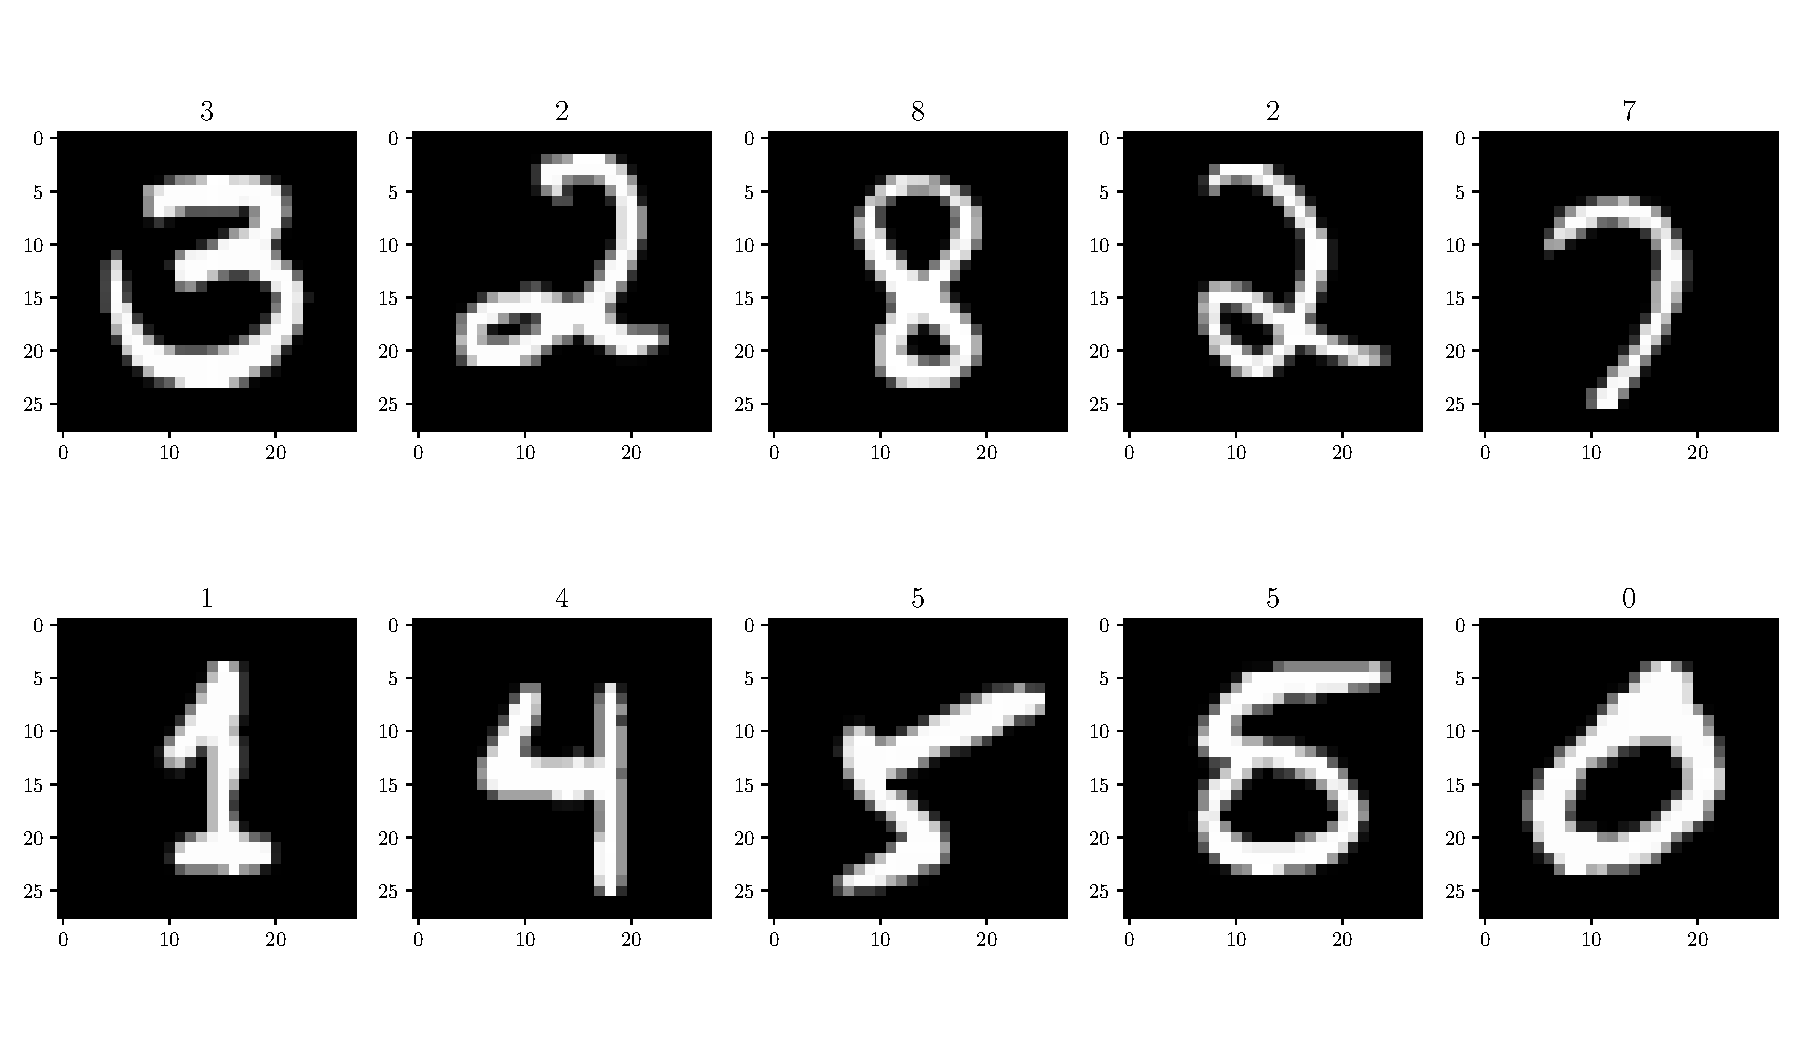
\includegraphics[width=.925\linewidth]{figures/mnist_28x28.pdf}
		\caption{Original data set of $28 \times 28$ images.}
		\label{fig:mnist_28x28}
	\end{subfigure}%
	\begin{subfigure}{.5\textwidth}
		\centering
		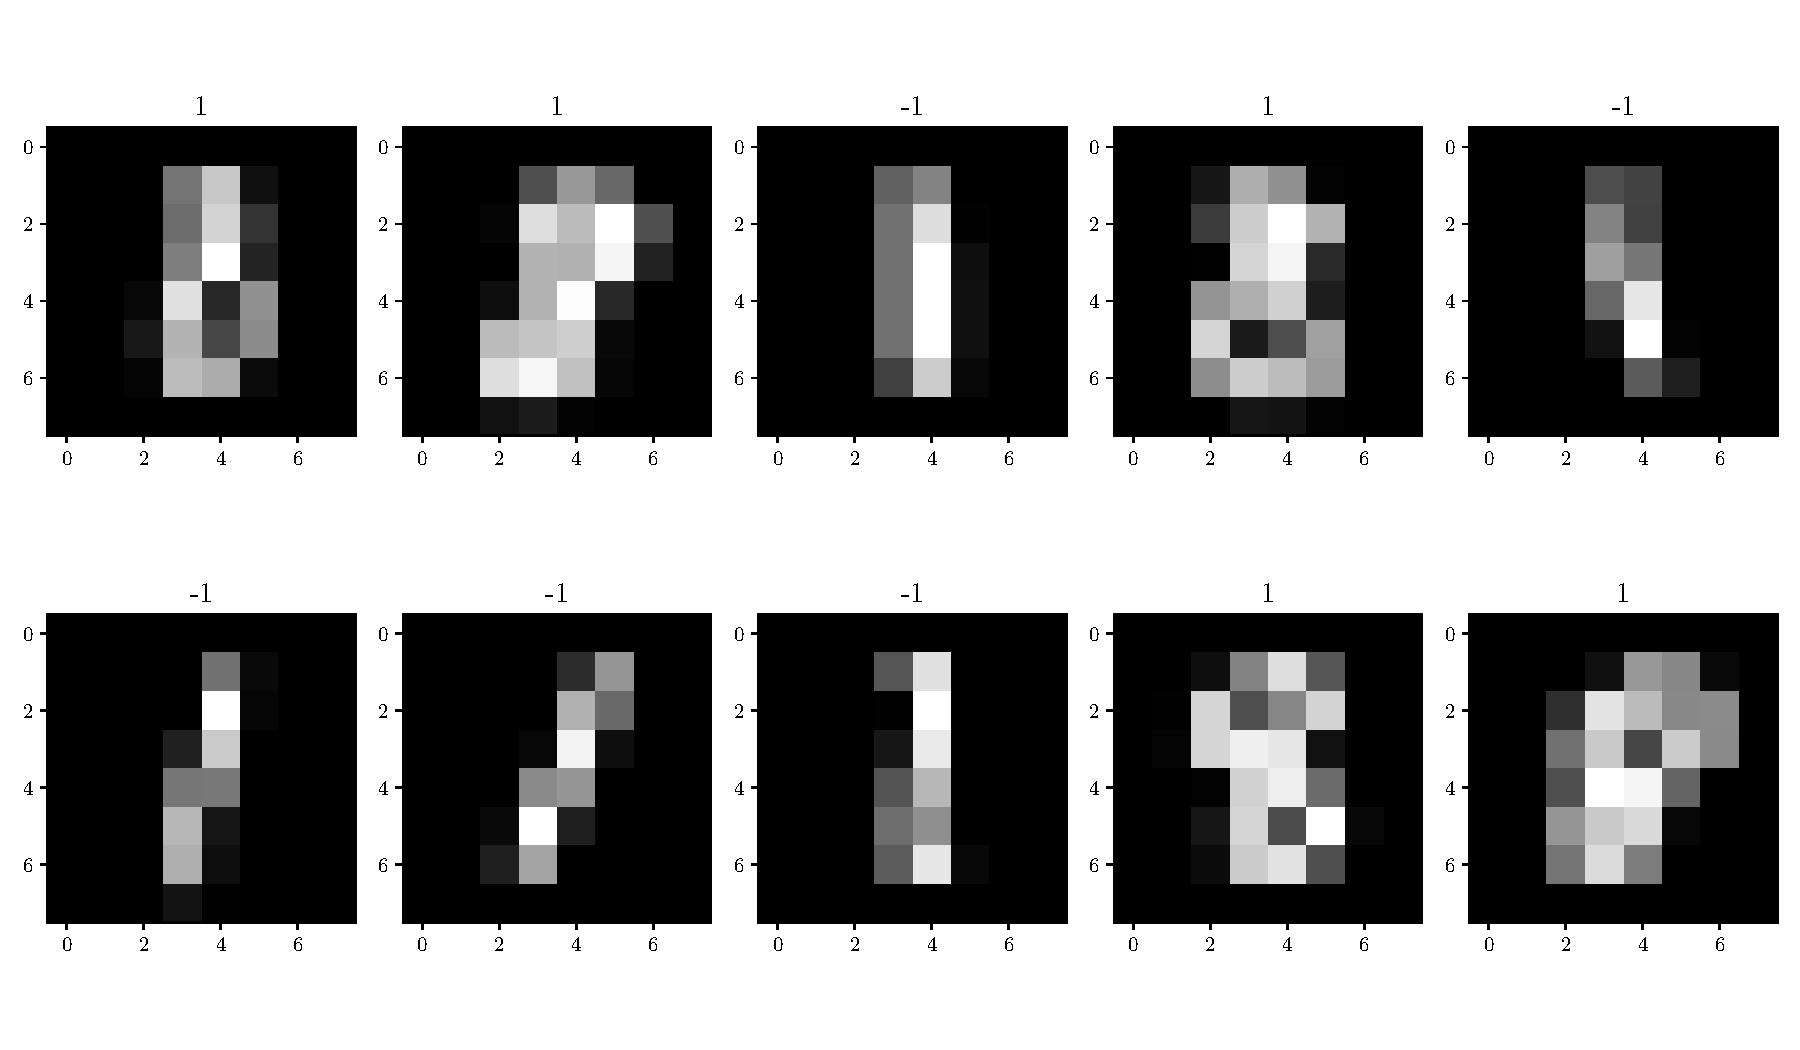
\includegraphics[width=.925\linewidth]{figures/mnist_8x8.pdf}
		\caption{Downsampled binary data set of $8 \times 8$ images.}
		\label{fig:mnist_8x8}
	\end{subfigure}
	\caption{Samples of the MNIST handwritten digits data set used for classification.}
	\label{fig:mnist}
\end{figure}

\subsubsection{Binary Downsampled Classifier} \label{sec:bdc}
The problem of supervised classification in machine learning is defined as follows: given a training set of data whose category is known, train a model which is able to identify to which category new data belongs.
A simple example that we will tackle in this section is recognizing if a handwritten digit is a 1 or an 8.

We implement a variational QNN to classify $8 \times 8$ images of handwritten digits (Figure~\ref{fig:mnist_8x8}).
It uses a quantum circuit together with a classical optimization algorithm to find the optimal parameters for the quantum circuit.
An overview of the quantum circuit used in the experiment can be found in Figure~\ref{fig:bdc-circuit}.
The variational QNN classifier learns as follows:
\begin{enumerate}
	\item Prepare data sample $\vec{x}$ in the amplitudes of a quantum state \ket{x}:
	\begin{equation}
	 \ket{x} = \dfrac{1}{\lVert\vec{x}\rVert}\sum_{i=0}^{N-1} x_i\ket{i},
	\end{equation}
	where \ket{i} represents the $i$'th computational basis state.
	\item Apply $L$ layers of parameterized unitaries: $\mathcal{U}(\vec{\theta})$\ket{x}, where $\mathcal{U}(\vec{\theta}) = U_\ell(\vec{\theta}_L) U_\ell(\vec{\theta}_{L-1}) \ldots U_\ell(\vec{\theta}_1)$.
	\item Measure expectation value $\expval{Z} = \bra{x}\mathcal{U}(\vec{\theta})^\dagger Z_n\, \mathcal{U}(\vec{\theta})\ket{x}$ of last qubit.
	\item Calculate and minimize loss $\mathcal{L}(\vec{\theta})$ through a classical optimization algorithm.
	\item Repeat until convergence.
\end{enumerate}
\begin{figure}[ht]
	\[
	\large
	\Qcircuit @C=1em @R=0.6em @!R {
		& & \multigate{4}{U_\ell(\vec{\theta}_1)} & \multigate{4}{U_\ell(\vec{\theta}_2)} & \qw & & \multigate{4}{U_\ell(\vec{\theta}_L)} & \qw & \qw \\
		& & \ghost{U_\ell(\vec{\theta}_1)} & \ghost{U_\ell(\vec{\theta}_2)} & \qw & & \ghost{U_\ell(\vec{\theta}_L)} & \qw & \qw \\
		\lstick{\ket{x}~~} & & \ghost{U_\ell(\vec{\theta}_1)} & \ghost{U_\ell(\vec{\theta}_2)} & \qw & & \ghost{U_\ell(\vec{\theta}_L)} & \qw & \qw \\
		& ~~\vdots & & & ~~\hdots & & & \vdots \\
		& & \ghost{U_\ell(\vec{\theta}_1)} & \ghost{U_\ell(\vec{\theta}_2)} & \qw & & \ghost{U_\ell(\vec{\theta}_L)} & \meter & \rstick{\expval{Z}} \cw
		\gategroup{1}{1}{5}{1}{.7em}{\{}
	}
	\]
	\caption{General circuit of the QNN\@. The network consists of $L$ layers with each layer implementing a parameterized unitary $U_\ell(\vec{\theta})$ whose parameters are optimized using a classical optimization algorithm. The decomposition of a layer is shown in Figure~\ref{fig:parametrized_unitary}.}
	\label{fig:bdc-circuit}
\end{figure}
For the binary classifier we use the square loss cost function:
\begin{equation}
\mathcal{L}(\vec{\theta}) = \sum_{i=1}^{D} \left(y_d - \bra{x_d}\mathcal{U}(\vec{\theta})^\dagger Z_n\, \mathcal{U}(\vec{\theta})\ket{x_d}\right)^2,
\end{equation}
where $D$ is the number of training samples and $y_d$ the correct label for input $x_d$.
Predicting the label $y$ for input $\vec{x}$ is done by taking the sign of the $Z$ expectation value of the last qubit:
\begin{equation}
y(\vec{x}) = \sign \left(\bra{x}\mathcal{U}(\vec{\theta})^\dagger Z_n\, \mathcal{U}(\vec{\theta})\ket{x}\right).
\end{equation}

We trained a QNN using a training set of 3148 images and a test set of 843 images.
As optimizer, we used mini-batch stochastic gradient descent (SGD) with a learning rate of $0.05$ and a batch size of $32$.
Due to computational limits, we restricted the initial experiment to 20 epochs.
After training for 20 epochs with 2 layers, it reached 97.2\% test accuracy without any hyperparameter tuning or circuit optimization.
The goal of this experiment is not to compete with classical state-of-the-art neural networks, which are capable of achieving an error percentage of only 0.23\% on multiclass classification of all the digits~(\cite{cirecsan2012multi}).\footnote{Which is not to say quantum neural networks can't compete with classical neural networks. In fact, \textcite{perez2019data} show a quantum classifier with two qubits to be at least comparable with classical methods by using data re-uploading techniques.}
Rather, it is meant to demonstrate the possibility of using quantum computers for machine learning problems and to hint that the universal approximation theorem~(\cite{csaji2001approximation}) applies to quantum neural networks.
It shows the potential to use quantum computers to process (quantum) data that classical computers cannot process efficiently.

\begin{figure}[ht]
	\[
	\large
	\Qcircuit @C=1em @R=0.6em @!R {
		& & \multigate{5}{U_\ell(\vec{\theta})} & \qw & & \gate{R_z(\theta_{1, 1})} & \gate{R_y(\theta_{1, 2})} & \gate{R_z(\theta_{1, 3})} & \ctrl{1} & \qw & \qw & \targ & \qw \\
		& & \ghost{U_\ell(\vec{\theta})} & \qw & & \gate{R_z(\theta_{2, 1})} & \gate{R_y(\theta_{2, 2})} & \gate{R_z(\theta_{2, 3})} & \targ & \ctrl{1} & \qw & \qw & \qw \\
		& & \ghost{U_\ell(\vec{\theta})} & \qw & & \gate{R_z(\theta_{3, 1})} & \gate{R_y(\theta_{3, 2})} & \gate{R_z(\theta_{3, 3})} & \qw & \targ & \qw & \qw & \qw \\
		& & & ~~= & & \vdots & \vdots & \vdots & & \vdots & & & & & \\
		& & \ghost{U_\ell(\vec{\theta})} & \qw & & \gate{R_z(\theta_{n-1, 1})} & \gate{R_y(\theta_{n-1, 2})} & \gate{R_z(\theta_{n-1, 3})} & \qw & \qw & \ctrl{1} & \qw & \qw  \\
		& & \ghost{U_\ell(\vec{\theta})} & \qw & & \gate{R_z(\theta_{n, 1})} & \gate{R_y(\theta_{n, 2})} & \gate{R_z(\theta_{n, 3})} & \qw & \qw & \targ & \ctrl{-5} & \qw
	}
	\]
	\caption{Decomposition of a layer $U_\ell(\vec{\theta})$. The amount of trainable parameters for a QNN with $n$ qubits and $L$ layers is $3n \cdot L$. The number of qubits required is decided by the dimension of the data: $n = \lceil \log_2N \rceil$, where $N$ is the input dimension. The downsampled MNIST classifier requires $\lceil \log_2(8 \cdot 8) \rceil = 6$ qubits.}
	\label{fig:parametrized_unitary}
\end{figure}

\subsubsection{One-vs-Rest Classifier}
To make a step into the direction of multi-class classification using a QNN, we first consider the problem of one-vs-rest classification.
We use the original $28 \times 28$ MNIST data set (Figure~\ref{fig:mnist_28x28}) to train a QNN to detect if a handwritten digit is 0 or not.
To encode a $28 \times 28$-dimensional image we need $\lceil \log_2(28 \cdot 28) \rceil = 10$ qubits.
As the complexity of the problem grows, we compare the performance of multiple optimizers: SGD, RMSprop, and Adam.
We also compare the performance with 2, 4 and 8 layers to see what impact increasing the number of layers has.
We trained the network for 30 epochs with a batch size of 32.
The training and testing data set consisted of 710 and 1372 images respectively.
Some hyperparameter tuning was done to find the optimal learning rate, but more tuning can be done to possibly increase performance.

The results of the experiment are shown in Figure~\ref{fig:ovr_results}.
In general, the performance of the classifiers seems to improve as we increase the number of layers, but ultimately it does not seem to benefit from more than 4 layers.
Adaptive learning rate methods RMSprop and Adam convergence faster and find a better optimum compared to vanilla SGD.
The amount of trainable parameters per network is 60 for 2 layers, 120 for 4 layers and 240 for 8 layers.
In contrast, a classical neural network has at least $28 \cdot 28 = 784$ parameters just for the input layer.

\begin{figure}[ht]
	\centering
	\begin{subfigure}{1\textwidth}
		\centering
		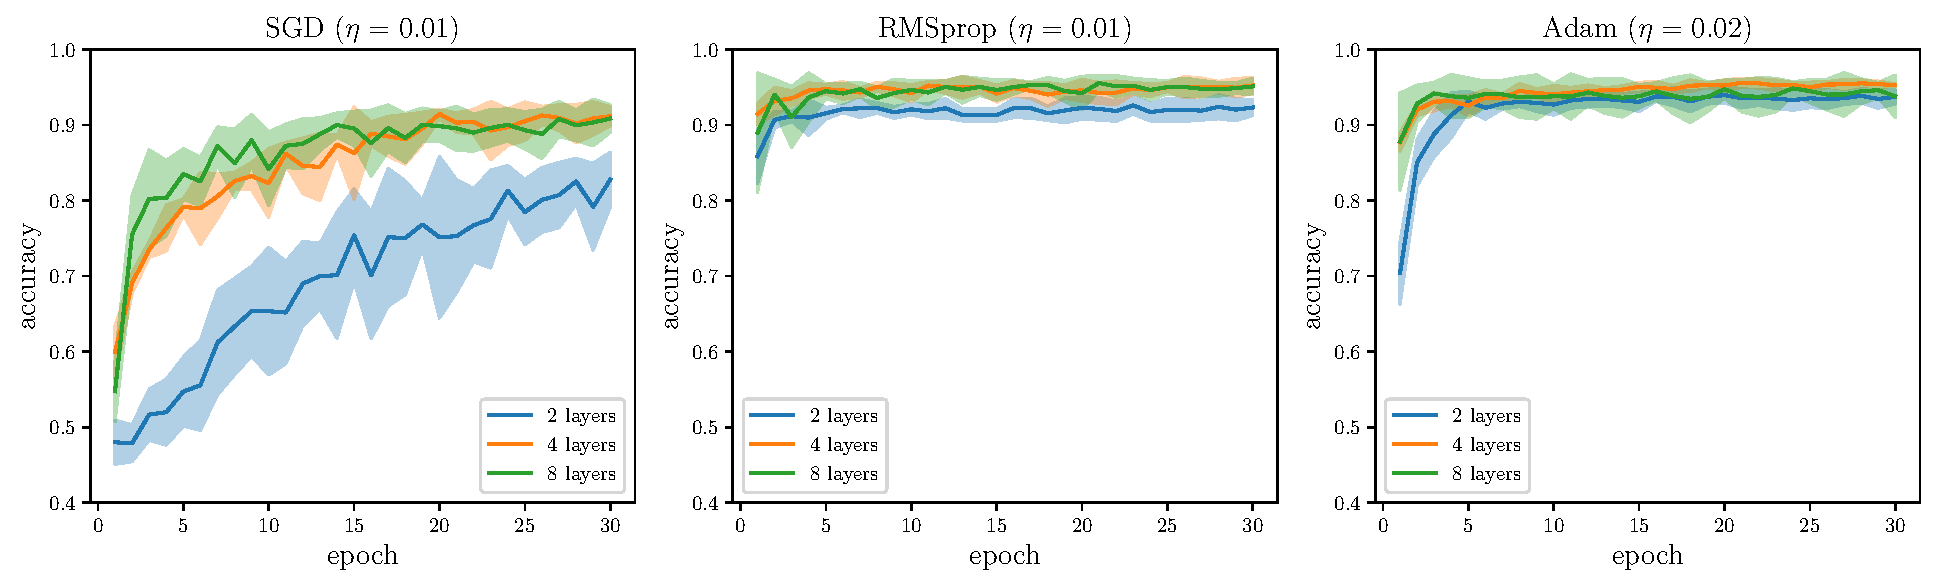
\includegraphics[width=1\linewidth]{figures/qnn_ovr_accuracy.pdf}
		\caption{Accuracy on test data set with different optimizers.}
		\vspace*{4mm}
	\end{subfigure}
	\begin{subfigure}{1\textwidth}
		\centering
		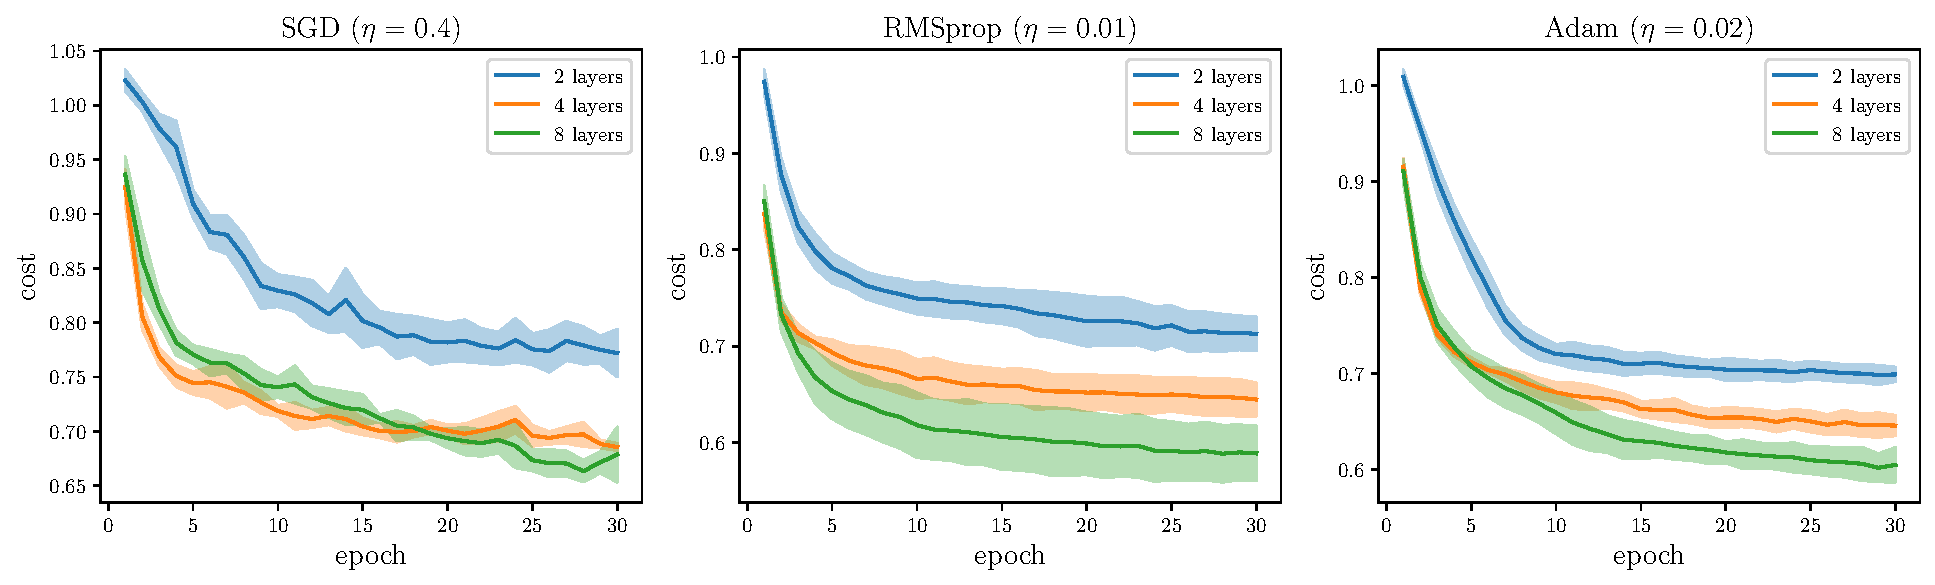
\includegraphics[width=1\linewidth]{figures/qnn_ovr_cost.pdf}
		\caption{Cost landscape of different optimizers.}
	\end{subfigure}
	\caption{Experimental results of a one-vs-rest QNN classifier for detecting if a handwritten digit is 0 or not. The data shown is the mean taken from five runs with the standard deviation plotted as the area under the mean.}
	\label{fig:ovr_results}
\end{figure}

\subsubsection{Multiclass Classifier} \label{sec:multiclass_classifier}
Finally we generalize the QNN classifier to a multiclass classifier by implementing a fidelity loss function as proposed by~\textcite{perez2019data}.
To implement this we need to make some changes to the QNN described in Section~\ref{sec:bdc}.
First, we introduce $C$ maximally orthogonal label states, where $C$ is the number of classes (Figure~\ref{fig:orthanogal_label_states}).
Then, instead of using the square loss function on the expectation value as cost, we measure the fidelity of the final state of the last qubit and the label state.
The goal then is to maximize the fidelity between the final state of the last qubit and the correct label state.
We define the fidelity cost function as following:
\begin{equation}
\mathcal{F}(\vec{\theta}) = - \dfrac{1}{D} \sum_{d=1}^{D} \log \left( \lvert \bra{y_d}\mathcal{U}(\vec{\theta})\ket{x_d} \rvert^2\right),
\end{equation}
where $D$ is the number of training samples, $\ket{y_d}$ the correct label state of input $\ket{x_d}$, and $\mathcal{U}(\vec{\theta})$ the parameterized layer unitaries.
To make a prediction, we measure the fidelities between the output and all the label states and choose the label with the highest fidelity.

We conduct a similar experiment to that from the previous section.
The problem at hand is to distinguish between the handwritten digits 1 through 6 including, giving six classes.
We take the six polar states $\{\ket{0}, \ket{1}, \ket{+}, \ket{-}, \ket{+i}, \ket{-i}\}$ as our maximally orthogonal label states (Figure~\ref{fig:orthanogal_label_states}).
The network was shown the training data set consisting of 27,009 samples once and was tested on 6009 samples.
The results are shown in Table~\ref{table:multiclass_results}.
All optimizers seem to perform relatively equal, with the adaptive optimizers finding a slightly better optimum with 10 layers.
We see a bigger performance increase when increasing the number of layers than before, likely due to the task at hand being more complex.
Due to the computational limits of quantum circuit simulation, the network was shown the dataset for only one epoch.
We predict the QNN's performance can be improved with more epochs, by redundantly encoding data and by using data re-uploading techniques as suggested by~\textcite{vidal2019input}~and~\textcite{perez2019data}.

\begin{table}[ht]
	\centering
	\begin{minipage}{.49\textwidth}
		\centering
		\contourlength{1.25pt}
		\begin{blochsphere}[radius=1.75cm, tilt=15, rotation=-20, opacity=0.1, color=white]
			\drawBallGrid[style={opacity=0.05}]{30}{30};
			
			\labelLatLon{zero}{90}{0};
			\labelLatLon{min}{0}{180};
			\labelLatLon{mini}{0}{90};
			\labelLatLon{plusi}{180}{90};
			\labelLatLon{plus}{0}{0};
			\labelLatLon{one}{-90}{90};
				
			\drawGreatCircle[style={opacity=0.4}]{0}{0}{0};
			\drawGreatCircle[style={opacity=0.4}]{90}{0}{0};
			\drawGreatCircle[style={opacity=0.4}]{90}{90}{90};
			
			\node[right=1mm] at (plusi) {\ket{+i}};
		
			\draw[opacity=0.4] (min) -- (plus);
			\draw[opacity=0.4] (mini) -- (plusi);
				
			\draw[color=red, line width=0.27mm, opacity=0.7] (zero) -- (plus);
			\draw[color=red, line width=0.27mm, opacity=0.7] (zero) -- (min);
			\draw[color=red, line width=0.27mm, opacity=0.7] (zero) -- (plusi);
			
			\draw[color=red, line width=0.27mm, opacity=0.7] (min) -- (plusi);
			
			\drawStateLatLon[statecolor=blue, statewidth=0.5pt, opacity=1]{state}{103}{-18};
			\node[left] at (state) {\ket{\psi}};
			
			\draw[color=red, line width=0.27mm, opacity=0.7] (zero) -- (mini);
			
			\draw[color=red, line width=0.27mm, opacity=0.7] (plus) -- (plusi);
			\draw[color=red, line width=0.27mm, opacity=0.7] (plus) -- (mini);
		
			\draw[color=red, line width=0.27mm, opacity=0.7] (min) -- (mini);
			
			\draw[color=red, line width=0.27mm, opacity=0.7] (one) -- (min);
			\draw[color=red, line width=0.27mm, opacity=0.7] (one) -- (plus);
			\draw[color=red, line width=0.27mm, opacity=0.7] (one) -- (mini);
			
			\node[above=1mm] at (zero) {\ket{0}};
			\node[left=1mm] at (min) {\ket{-}};
			\node[left] at (mini) {\contour{black!9}{\ket{-i}}};
			\node[right=1mm] at (plus) {\ket{+}};
	
			\node[below=1mm] at (one) {\ket{1}};
		\end{blochsphere}
		\captionof{figure}{Bloch sphere representation of six maximally orthogonal points which are used as labels. The circuit output state \ket{\psi} would get classified to the class corresponding to the label state \ket{0}, as their fidelity $\lvert\ip{0}{\psi}\rvert^2$ is the largest.}
		\label{fig:orthanogal_label_states}
	\end{minipage}
	\hfill
	\begin{minipage}{.475\textwidth}
		\centering
		{\renewcommand{\arraystretch}{1.2}
		\begin{tabular}{ c|c|c } 
			\hline
			Optimizer & Layers & Test accuracy \\
			\hline
			\multirow{4}{5em}{SGD ($\eta = 0.4$)} & 2 & $44.6\% \pm 0.019$ \\ 
			& 4 & $67.8\% \pm 0.026$ \\ 
			& 8 & $70.7\% \pm 0.009$ \\
			& 10 & $72.6\% \pm 0.026$ \\
			\hline
			\multirow{4}{5em}{RMSprop ($\eta = 0.01$)} & 2 & $49.5\% \pm 0.039$ \\ 
			& 4 & $66.8\% \pm 0.023$ \\ 
			& 8 & $70.8\% \pm 0.038$ \\
			& 10 & $74.9\% \pm 0.012$ \\
			\hline
			\multirow{4}{5em}{Adam ($\eta = 0.02$)} & 2 & $45.9\% \pm 0.025$ \\ 
			& 4 & $68.9\% \pm 0.012$ \\ 
			& 8 & $71.6\% \pm 0.030$ \\
			& 10 & $74.4\% \pm 0.022$ \\
			\hline
		\end{tabular}
		}
		\caption{Quantum neural network performance on multiclass classification of six classes. The accuracy is taken as the mean of five repeated runs.}
		\label{table:multiclass_results}
	\end{minipage}
\end{table}


\subsubsection{Regression Results} \label{sec:qnn-regression}
We take on the problem of learning the functions $x^3$, $\cos(\pi x)\sin(2\pi x + 2)$, $|x|$ and $e^x$ to demonstrate the QNN's ability of representing non-linear real functions.
The network is shown 75 samples of the functions in the range $[-1, 1]$ from a uniform distribution and is tested on 100 evenly spaced numbers over the same interval.
The data of the functions are one-dimensional, and we employ a data re-uploading technique described by \textcite{perez2019data} to achieve generalization with a small number of qubits (Figure~\ref{fig:data-reuploading-circuit}).
\begin{figure}[ht]
	\[
	\large
	\Qcircuit @C=1em @R=0.6em @!R {
		\lstick{\ket{0}} & \multigate{3}{U_\Phi(x)} & \multigate{3}{U_\ell(\vec{\theta}_1)} & \qw & & \multigate{3}{U_\Phi(x)} & \multigate{3}{U_\ell(\vec{\theta}_L)} & \qw & \qw \\
		\lstick{\ket{0}} & \ghost{U_\Phi(x)} & \ghost{U_\ell(\vec{\theta}_1)} & \qw & & \ghost{U_\Phi(x)} & \ghost{U_\ell(\vec{\theta}_L)} & \qw & \qw \\
		~~\vdots & & & ~~\hdots & & & & \vdots \\
		\lstick{\ket{0}} & \ghost{U_\Phi(x)} & \ghost{U_\ell(\vec{\theta}_1)} & \qw & & \ghost{U_\Phi(x)} & \ghost{U_\ell(\vec{\theta}_L)} & \meter & \rstick{\expval{Z}} \cw
	}
	\]
	\caption{Data re-uploading QNN circuit used to achieve generalization with a small amount of qubits. $U_\ell$ represents a layer as before in Section~\ref{sec:bdc}, and $U_\Phi$ represents the unitary that encodes the input data in the quantum state. In our example we use one-dimensional data, but $U_\Phi$ can be extended to encode a high-dimensional vector.}
	\label{fig:data-reuploading-circuit}
\end{figure}

\noindent
Every layer before applying a parameterized unitary $U_\ell(\vec{\theta})$, we encode a data point $x$ in $n$ qubits as follows:
\begin{equation} \label{eq:regression_encode}
U_\Phi(x) = \bigotimes_{i=1}^{n}R_y^{(i)}(\arccos x)R_y^{(i)}(\arcsin x).
\end{equation}
The whole circuit can then be described as
\begin{equation}
\mathcal{U}(\vec{\theta}, x) = U_\ell(\vec{\theta}_L)U_\Phi(x) U_\ell(\vec{\theta}_{L-1})U_\Phi(x) \ldots U_\ell(\vec{\theta}_1)U_\Phi(x),
\end{equation}
and the network's output is given by
\begin{equation}
y(x) = \gamma \cdot \bra{0}\mathcal{U}(\vec{\theta}, x)^\dagger Z_n\, \mathcal{U}(\vec{\theta}, x)\ket{0}.
\end{equation}
Here, $\gamma$ is a trainable parameter initialized to 1.
We use the mean squared error as cost function.
\begin{figure}[ht]
	\centering
	\begin{subfigure}{.4875\textwidth}
		\centering
		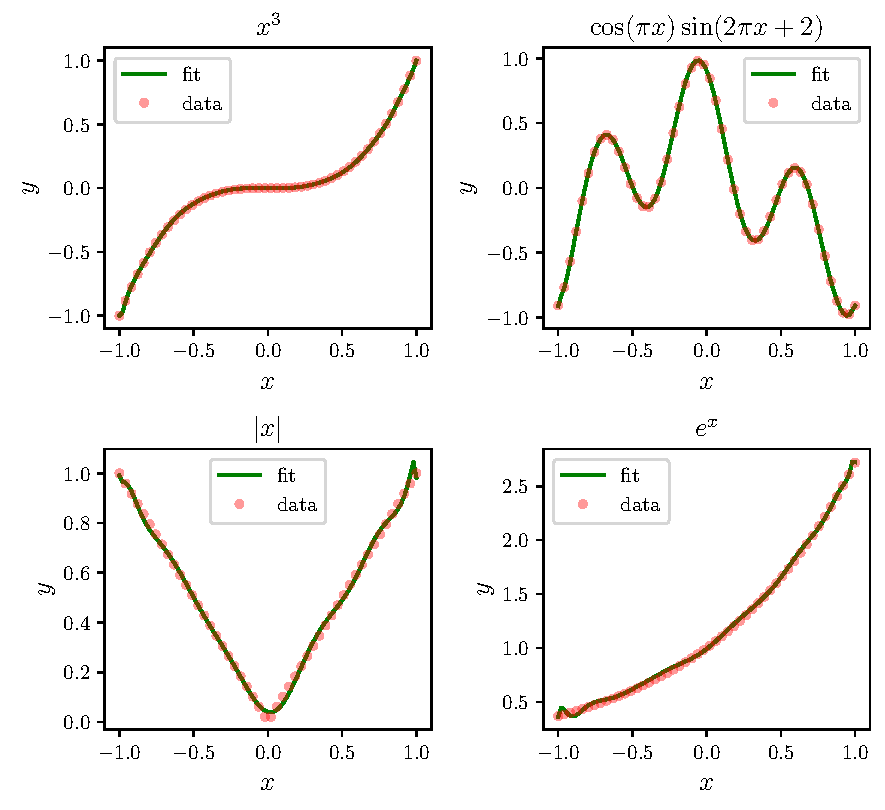
\includegraphics[width=1\linewidth]{figures/qnn_regression.pdf}
		\caption{Teacher data vs. learned function. The red points represent the teacher data shown to the network, and the green line represents the learned function.}
	\end{subfigure}
	\hfill
	\begin{subfigure}{.4875\textwidth}
		\centering
		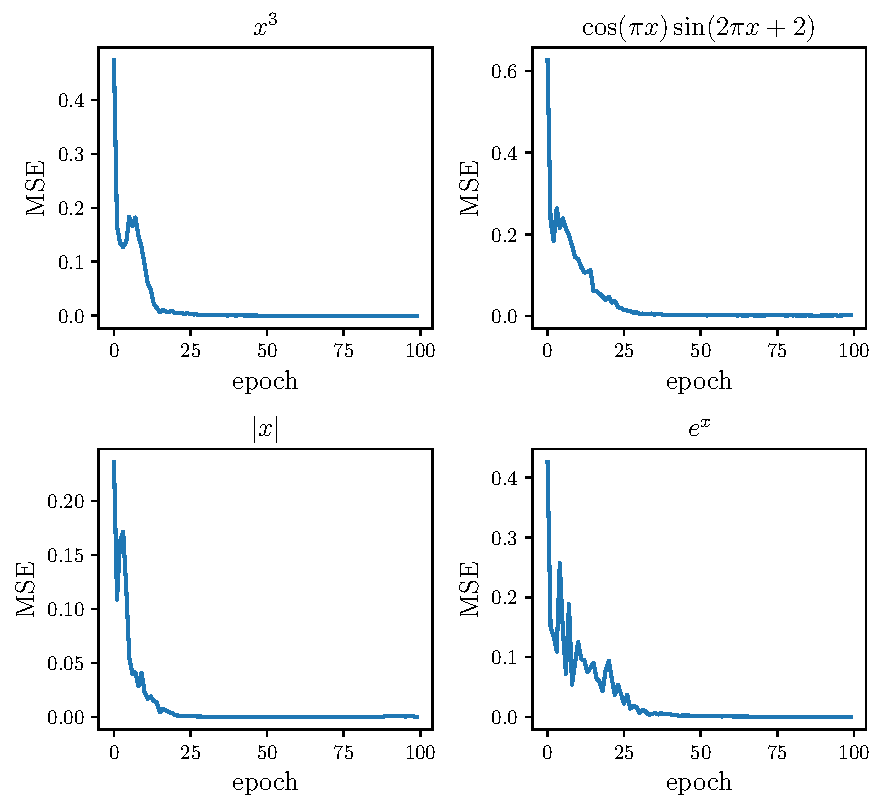
\includegraphics[width=1\linewidth]{figures/qnn_regression_mse.pdf}
		\caption{Landscapes of mean squared error cost function. The QNNs were trained for 100 epochs with 3 layers. RMSprop was used as optimizer with learning rate 0.01 and momentum 0.9.}
	\end{subfigure}
	\caption{Performance of our QNN learning continuous functions. Input data was encoded in three qubits according to Equation~\ref{eq:regression_encode}.}
	\label{fig:qnn_regression_results}
\end{figure}

The results are shown in Figure~\ref{fig:qnn_regression_results}.
We see that the QNN has an easy time learning the wavelike functions $x^3$ and $\cos(\pi x)\sin(2\pi x + 2)$ due to the encoding method.
The other functions $|x|$ and $e^x$ are approximated well, but leave room for improvement.
Possible improvement can be made by employing better (problem specific) encoding techniques and more hyperparameter tuning.
We have demonstrated a naive approach to doing regression tasks using our QNN.
Nevertheless, we managed to train models that approximate these non-linear functions well.

\subsubsection{Discussion and Further Work}
We have described and implemented a variational QNN capable of classifying classical data and doing simple regression tasks.
By applying the QNN to the problem of handwriting recognition, we have demonstrated its capability of solving real-world problems.
Our QNN exploits the exponential Hilbert space of quantum states to encode classical data in an amount of qubits logarithmic to the input data's dimension.
This demonstrates the possibility to process high dimensional (quantum) data that is intractable for classical computers to process.
In Appendix~\ref{sec:classification-other} we apply the QNN classifier on other data sets to show its ability to adapt to various problems.

Further work can be done by using more quantum-specific optimization methods~(\cite{stokes2019quantum}), optimizing the measuring of expectation values~(\cite{sweke2019stochastic}), improving the circuit initialization strategy~(\cite{mcclean2018barren}), conducting more experiments on quantum and classical data, defining useful benchmarks and experimenting with real quantum hardware.
Improvements can also be made to the encoding of classical data into a quantum Hilbert space by experimenting with different feature maps (\cite{schuld2019quantum}).

\section{Conclusion} \label{sec:conclusion}
Machine learning is ubiquitous and widely used to perform complex tasks such as image recognition, playing games, recognizing speech and more.
Recently, researchers have been looking for ways to apply quantum computers to machine learning, resulting in the field of quantum machine learning.
Quantum machine learning is an exciting new field that shows the potential to speed up certain machine learning algorithms by using quantum computers.
However, most known QML algorithms require a large amount of quantum resources and cannot be implemented on the NISQ devices we will have access to in the near future.
This has caused much research to shift towards the development of variational algorithms, which involve a small quantum subroutine run inside of a classical optimization loop, removing the need for a large-scale, coherent quantum computer. 
Though it is likely that most QML approaches will not be of much practical use in the near future, variational algorithms might already provide a quantum advantage at the level of 50-100 qubits for certain problems.
However, we should not expect the promised exponential speedups to be achieved on near-term devices.
In this report we implemented a variational QNN using quantum circuit simulation to demonstrate how quantum computers can be used to solve machine learning problems.
We hope this work will somewhat help advance the field of QML and make QML more accessible to researchers around the world.
There is still much work to be done in both implementation and theory, but the work done so far is promising.
Quantum computing may very well solve some of the computational problems we are facing today and revolutionize the field of machine learning.

\clearpage

\printbibliography[heading=bibintoc]

\clearpage

\begin{appendices}
\section{Classification Results on Other Data} \label{sec:classification-other}
We showed that our QNN classifier is capable of classifying handwritten digits.
Here, we apply the QNN described in Section~\ref{sec:multiclass_classifier} to more data sets to see its performance on other problems.
With this, we aim to show that the classifier is able to adapt to a broad variety of problems.
We test our QNN on three different data sets, generated by the scikit-learn~(\cite{scikit-learn}) functions \verb|make_moons|, \verb|make_circles| and \verb|make_classification| with a noise factor of 0.125.
The data sets consist of 300 entries, of which 75\% was used as training data and 25\% as testing data.
A data point is two-dimensional with values in $[-1.5, 1.5]$ and has a binary label 0 or 1.
It is encoded into a quantum state by single-qubit rotations instead of amplitude encoding.
Because of the low dimensional data, we redundantly encode it once in an extra qubit, resulting in a two-qubit classifier.
A data point $(\begin{matrix}x_1 & x_2\end{matrix})$ is encoded in the two qubits as $\bigotimes_{i=1}^{n}R_y^{(i)}(x_1)R_z^{(i)}(x_2)$.
We also use the data re-uploading technique described in Section~\ref{sec:qnn-regression} to achieve generalization with just two qubits.

The results are plotted in Figure~\ref{fig:classification_decision_regions}.
In all cases, the QNN approximates the function well.
We can see that increasing the number of layers allows the network to learn more complex shapes, but even with 2 layers it finds the desired shape.
Note that due to the encoding method and the non-linear behavior of rotation gates, the QNN has an easy time finding wavelike patterns in data.

\begin{figure}[ht]
	\centering
	\begin{subfigure}{.9458\textwidth}
		\centering
		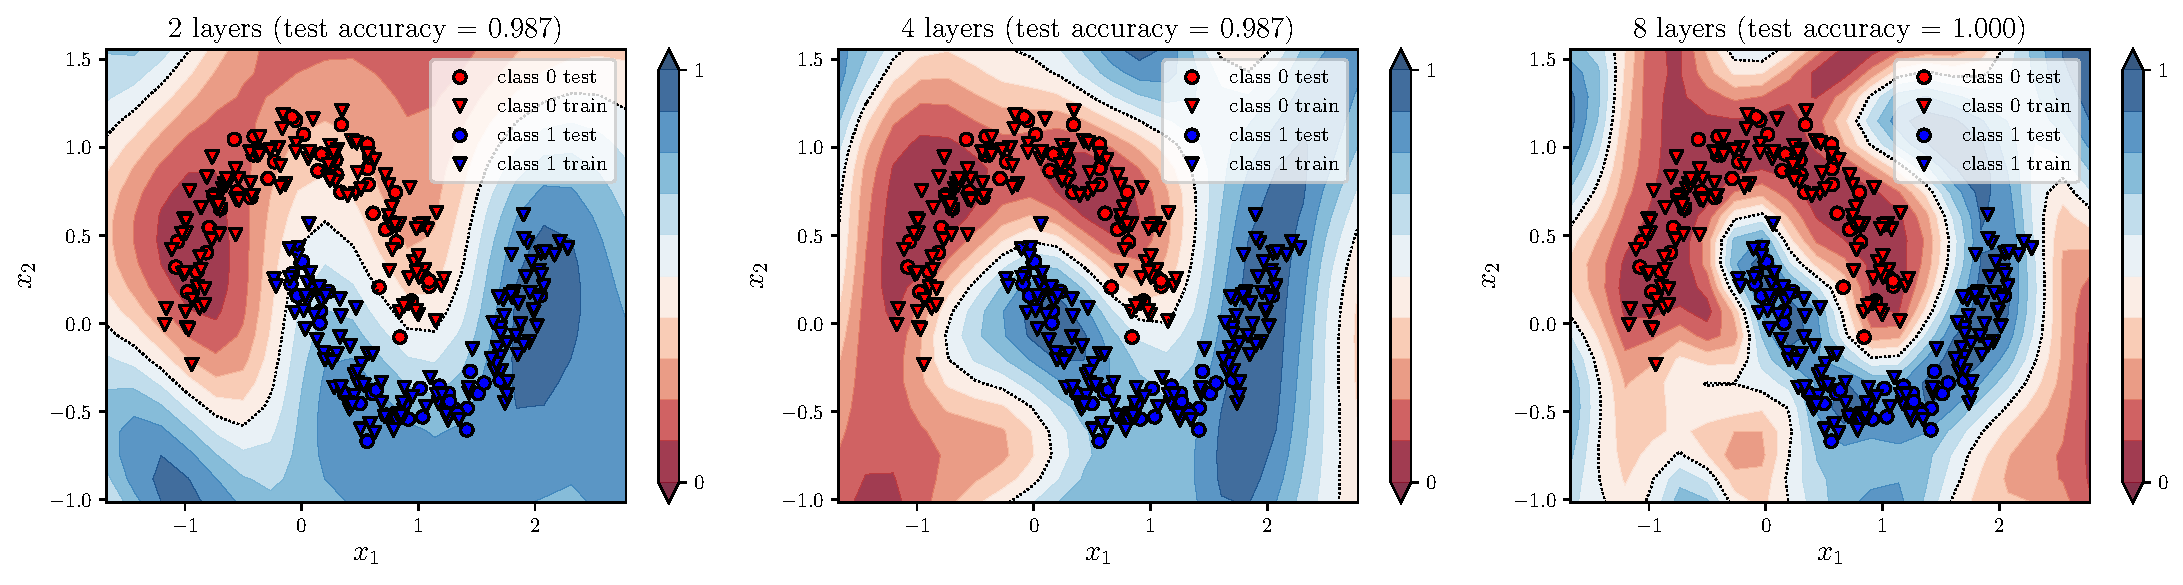
\includegraphics[width=1\linewidth]{figures/qnn_moons_classification.pdf}
	\end{subfigure}
	\begin{subfigure}{.9458\textwidth}
		\centering
		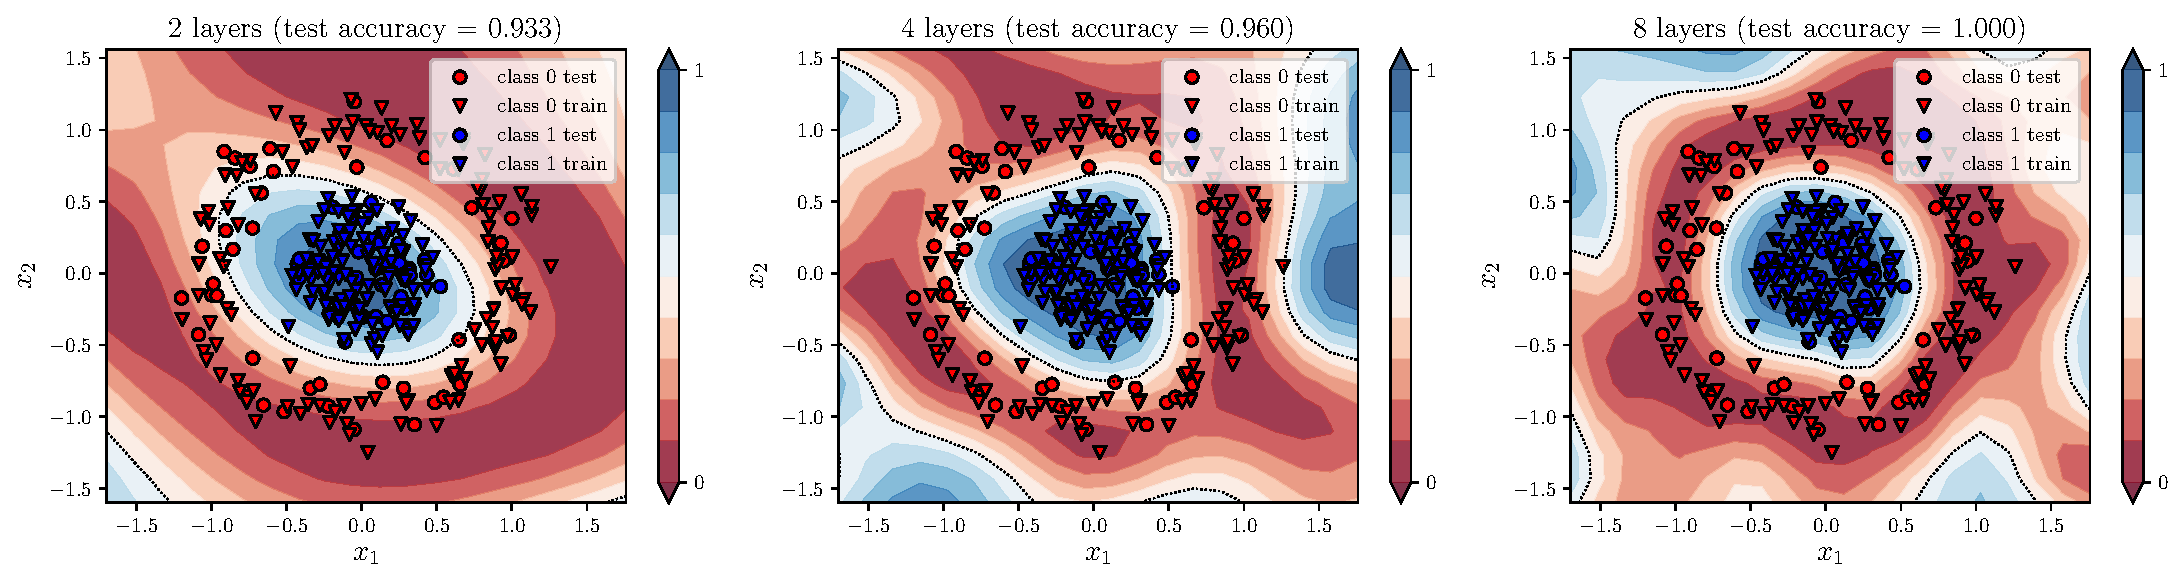
\includegraphics[width=1\linewidth]{figures/qnn_circles_classification.pdf}
	\end{subfigure}
	\begin{subfigure}{.9458\textwidth}
		\centering
		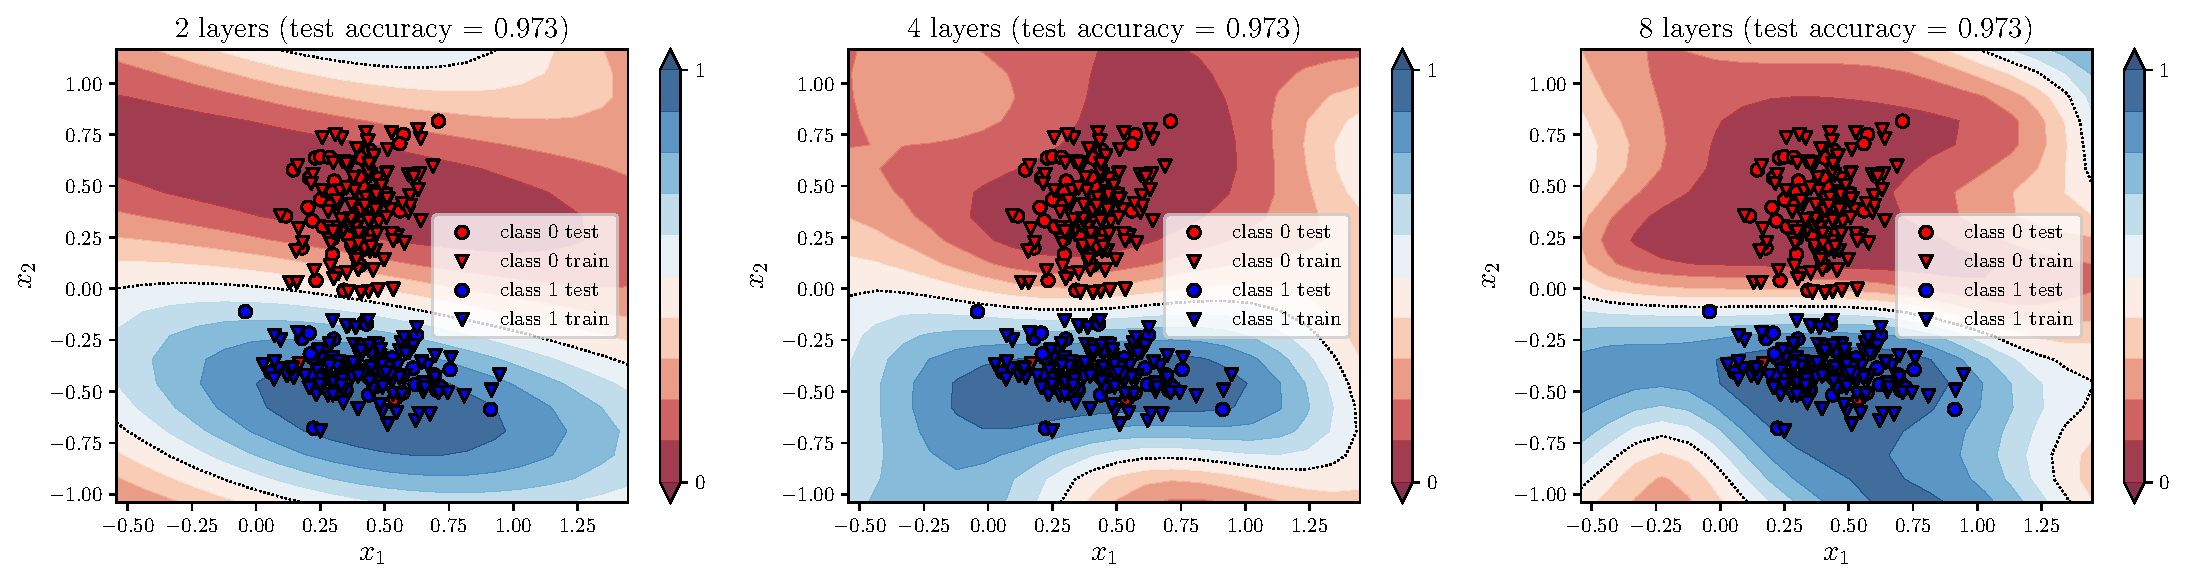
\includegraphics[width=1\linewidth]{figures/qnn_linear_classification.pdf}
	\end{subfigure}
	\cprotect\caption{Classification results of a two-qubit QNN on the \verb|make_moons| (top row), \verb|make_circles| (middle row) and \verb|make_classification| (bottom row) data sets. All networks were trained for 10 epochs using RMSprop as optimizer with learning rate 0.05 and momentum 0.5. The red and blue contours represent the certainty of classifying 0 and 1 respectively.}
	\label{fig:classification_decision_regions}
\end{figure}

\section{CPU and GPU Simulation Benchmarks} \label{sec:cpu-gpu-benchmark}
Quantum circuit simulation is known to be exponentially hard on classical computers.
The state space of a quantum system grows exponentially with the number of particles, making simulation of higher amount of particles intractable on a classical computer.
To make our simulations as efficient as possible, we compare the performance of the Qulacs simulator on CPU and GPU.
We run the benchmarks on the Lisa system of SURFsara.
The node used has Intel Xeon Gold 6126 CPUs at 2.60GHz and an NVIDIA TITAN RTX GPU.

We measure how the execution time increases as the amount of qubits increases.
The measure we test is 100 executions of 4 layers of the circuit described in Figure~\ref{fig:parametrized_unitary}.
The parameters are randomly generated from a uniform distribution.
We also measure $\expval{Z}$ every iteration and compare the results of the GPU simulation with the CPU simulation to make sure they agree.
The results are visualized in Figure~\ref{fig:qulacs_benchmark}.
We can see that increasing the number of cores improves simulation times for higher number of qubits.
For qubit counts from 18 and higher, GPU simulation is much more efficient.
If we look at Table~\ref{table:qulacs_benchmark_results}, we see that single-core CPU simulation is most efficient up to 12 qubits.
While GPU always seems to beat multiple cores, running on a large number of cores is a good alternative if there is no GPU available.

\begin{figure}[ht]
	\centering
	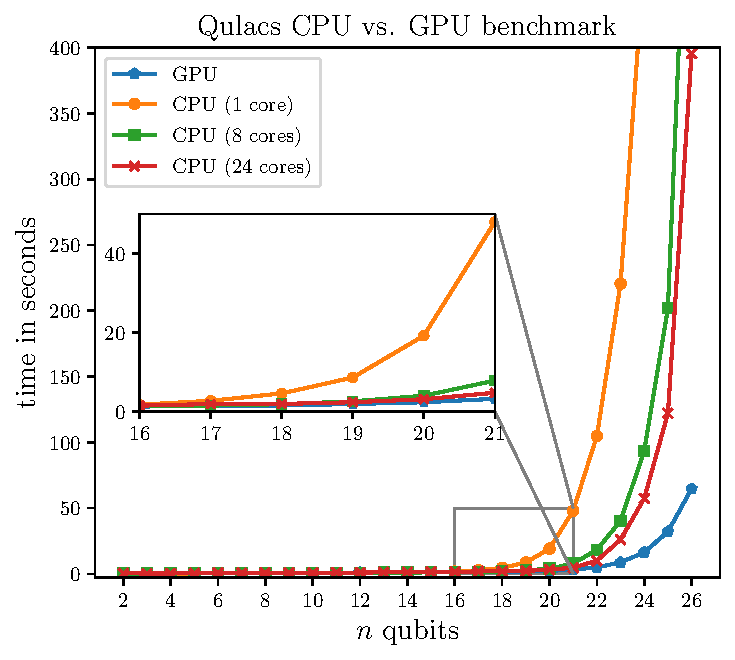
\includegraphics[width=0.625\linewidth]{figures/qnn_cpu_vs_gpu.pdf}
	\captionof{figure}{Comparison of quantum simulation runtime between CPU and GPU.}
	\label{fig:qulacs_benchmark}
\end{figure}

\begin{table}[ht]
	\centering
	{\renewcommand{\arraystretch}{1.1}
		\begin{tabular}{ c|c|c|c|c|c } 
			\hline
			$n$ qubits & GPU & CPU (1 core) & CPU (8 cores) &  CPU (24 cores) & CPU (48 cores) \\
			\hline
			2 & 0.292s & \textbf{0.145s} & 0.161s & 0.223s & 0.236s \\
			4 & 0.435s & \textbf{0.253s} & 0.258s & 0.279s & 0.297s \\
			6 & 0.605s & \textbf{0.389s} & 0.393s & 0.428s & 0.458s \\
			8 & 0.750s & \textbf{0.492s} & 0.497s & 0.544s & 0.578s \\
			10 & 0.914s & \textbf{0.615s} & 0.616s & 0.667s & 0.716s \\
			12 & 1.087s & \textbf{0.742s} & 0.762s & 0.834s & 0.926s \\
			14 & 1.261s & 0.975s & \textbf{0.958s} & 1.041s & 1.135s \\
			16 & 1.534s & 1.595s & \textbf{1.218s} & 1.238s & 1.292s \\
			18 & \textbf{1.746s} & 4.111s & 2.030s & 1.763s & 1.762s \\
			20 & \textbf{2.610s} & 18.232s & 4.836s & 3.357s & 3.011s \\
			22 & \textbf{5.208s} & 125.588s & 19.282s & 11.283s & 9.023s \\
			24 & \textbf{16.689s} & 640.009s & 99.339s & 84.670s & 71.659s \\
			26 & \textbf{65.671s} & 3245.341s & 444.671s & 359.843s & 399.357s \\
			\hline
		\end{tabular}
	}
	\caption{Qulacs quantum circuit simulator benchmark results. The fastest result per $n$ qubits is shown in bold.}
	\label{table:qulacs_benchmark_results}
\end{table}

\end{appendices}

\end{document}